\section{Installation de SiCP2}
%
\subsection{Exécutable pour Windows}
%
\begin{center}
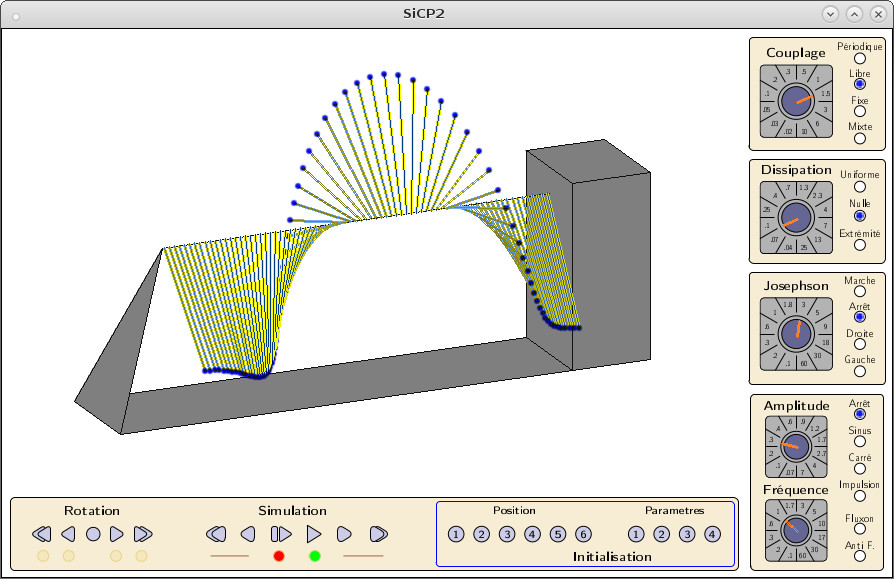
\includegraphics[width=.9\textwidth]{./illustration/SiCP2}
\end{center}
%
https://github.com/Cphysique/SiCP2/
https://cphysique.github.io/
%
\subsection{Compilation du code source}
%
Le bouton vert de la page 
%
\begin{center}
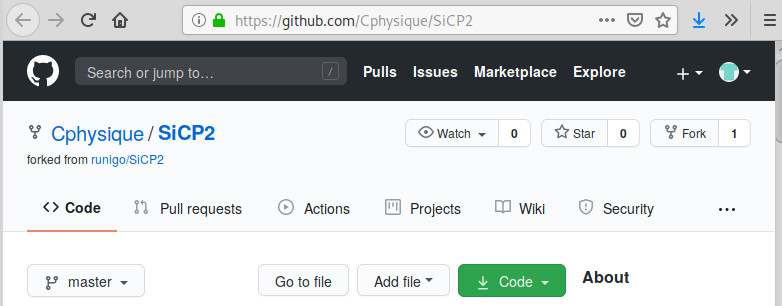
\includegraphics[width=.9\textwidth]{./presentation/CphysiqueSiCP2}
\end{center}
%
%
\begin{center}
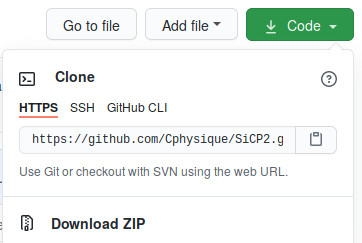
\includegraphics[width=.9\textwidth]{./presentation/CphysiqueSiCP2code}
\end{center}
%
Cette section traite de l'installation des simulateurs SiTS2, SiCF2 et SiCP2 sur un système d'exploitation de type debian. Le téléchargement se fait avec un navigateur internet, la compilation et l'exécution se font dans un terminal. L'installation des outils de compilation nécessite les privilèges du super-utilisateur.
\begin{itemize}[leftmargin=1cm, label=\ding{32}, itemsep=0pt]
\item {\bf Installation des outils de compilation}
Avec les droits du super-utilisateur
	\begin{itemize}[leftmargin=1cm, label=\ding{32}, itemsep=0pt]
	\item \texttt{apt-get install gcc make libsdl-dev}
	\item Pour les versions 2 des simulateurs, installer la librairie SDL2 :
	\item \texttt{apt-get install libsdl2-dev}
	\end{itemize}
\item {\bf Téléchargement des sources}
	\begin{itemize}[leftmargin=1cm, label=\ding{32}, itemsep=0pt]
	\item Télécharger les fichiers \texttt{.zip} sur github
		\begin{itemize}[leftmargin=1cm, label=\ding{32}, itemsep=0pt]
		\item \texttt{https://github.com/runigo/SiCP2/archive/master.zip}
		\item \texttt{https://github.com/runigo/SiCF2/archive/master.zip}
		\item \texttt{https://github.com/runigo/SiTS2/archive/master.zip}
		\end{itemize}
	\item Décompresser les fichiers \texttt{.zip}
		\begin{itemize}[leftmargin=1cm, label=\ding{32}, itemsep=0pt]
		\item \texttt{unzip SiCP2-master.zip}
		\item \texttt{unzip SiCF2-master.zip}
		\item \texttt{unzip SiTS2-master.zip}
		\end{itemize}
	\end{itemize}
\item {\bf Compilation}
	\begin{itemize}[leftmargin=1cm, label=\ding{32}, itemsep=0pt]
	\item La commande \texttt{make} dans le répertoire des sources produit un fichier exécutable :
		\begin{itemize}[leftmargin=1cm, label=\ding{32}, itemsep=0pt]
		\item \texttt{SiCP2} pour SiCP
		\item \texttt{SiCF2} pour SiCF
		\item \texttt{SiTS2} pour SiTS
		\end{itemize}
	\end{itemize}
%
\item {\bf Exécution}
	\begin{itemize}[leftmargin=1cm, label=\ding{32}, itemsep=0pt]
	\item En ligne de commande, avec d'éventuelles options
		\begin{itemize}[leftmargin=1cm, label=\ding{32}, itemsep=0pt]
		\item \texttt{./SiCP2 [OPTION]}
		\item \texttt{./SiCF2 [OPTION]}
		\item \texttt{./SiTS2 [OPTION]}
		\end{itemize}
	\item La fenêtre graphique donne une représentation de la simulation,
	\item Le terminal affiche les informations.
	\end{itemize}
\end{itemize}

%%%%%%%%%%%%%%%%%%%%%%%%%%%%%%%%%%%%%%%%%%%%%%%%%%%%%%%%%%%%%%%%%%%%%%%%%%%%%%%%%%%%%%%%%%%%%
